%\begin{center}
%\large \bf \runtitulo
%\end{center}
%\vspace{1cm}
\section{Motivación}
Las historias clínicas orientadas a problemas monitorizan y detallan una lista de problemas médicos para cada paciente, que incluyen  tanto el diagnóstico final como todos aquellos hallazgos que aún no han sido específicamente diagnosticados \cite{Weed1968}. La lista está separada en problemas activos y pasivos. Los problemas activos deben representar la situación actual del paciente, dándole al médico una herramienta para la toma de decisiones sobre el tratamiento a seguir. Una vez que se ha establecido la lista actualizada de problemas, todas las subsecuentes órdenes, planes, notas de progreso y datos numéricos deben ser asociados a cada problema. Inherente a este enfoque está la necesidad de completitud y actualización en la formulación de la lista de  problemas. Esto requiere que los datos sean apropiadamente recolectados y actualizados de activos a pasivos, de tal manera que las conclusiones que emergen a partir de los datos sean lógicas y relevantes. Otra necesidad es la exactitud e integridad con la que los problemas son definidos inicialmente y esto tiene relación directa con la granularidad con la que se seleccionan los problemas \cite{Luna2013}. 
 
El \textit{Institute of Medicine (IOM)}\footnote{El \textit{Institute of Medicine (IOM)} es una organización independiente y sin ánimo de lucro fundada en 1970 como el brazo de la salud de la Academia Nacional de las Ciencias de Estados Unidos. Su objetivo es ayudar a sectores de gobierno y privado a tomar decisiones de salud informadas al proporcionar evidencia confiable} y la \textit{Joint Commission}\footnote{La \textit{Joint Commission} es una organización independiente y sin ánimo de lucro que acredita y certifica más de 20.500 organizaciones y programas de salud en Estados Unidos. La acreditación y certificación \textit{Joint Commission} es reconocida a nivel mundial como un símbolo de calidad que refleja el compromiso de la organización para cumplir con ciertos estándares de desempeño.} recomiendan que la lista de problemas sea exacta, actualizada y completa. Éstas se han convertido en la característica más importante para medir su calidad, ya que una lista de problemas actualizada y con un nivel adecuado de detalles mejora la comunicación entre profesionales de la salud, y se espera que también mejore la calidad en la atención a los pacientes. La exactitud en la lista de problemas impacta directamente en los sistemas de toma de decisiones del hospital y en la implementación de sus  programas de salud. Sin embargo, a pesar de los numerosos beneficios, las listas de problemas son a menudo imprecisas, incompletas y desactualizadas ya que no representan la situación actual del paciente.
 
La \acrfull{HCE} del \acrfull{HIBA} utiliza  listas de problemas como componente estructural, y se han podido identificar deficiencias en la completitud, actualización y exactitud \cite{Otero2014}. A pesar de que implementa Snomed CT\footnote{http://www.ihtsdo.org/} como terminología clínica de referencia para identificar los problemas, su gran tamaño es también un obstáculo para su uso y mantenimiento. Existe evidencia que indica que se está utilizando sólo una pequeña fracción de su contenido \cite{Lezcano2011}. Además, un estudio concluyó que en las áreas de hospitalización, emergencia y ambulatorios, los problemas registrados por los profesionales en la atención primaria de salud tienen mejor calidad que los registrados por los especialistas, y sugiere que trabajar con interfaces orientadas al contexto mejora la exactitud \cite{Luna2013}. 
 
El desarrollo de esta tesis propone un enfoque basado en la teoría de grafos para agrupar los conceptos de Snomed CT que se utilizan en la composición de las listas de problemas del \acrshort{HIBA}. Se analiza y evalúa la calidad de los grupos generados automáticamente en relación a diferente información contextual como el ámbito (internación, ambulatorios, emergencia y atención domiciliaria), el servicio de atención de la salud y el grupo etario del paciente. A partir de las relaciones de estos grupos se construye una taxonomía complementaria para clasificar los problemas de una manera que sea consistente con su uso dentro de la \acrshort{HCE}.
 
La taxonomía  de los problemas tiene un impacto directo en la organización de los datos y permite la creación de servicios de búsqueda para recuperar problemas basados en el contexto y en la co-ocurrencia de problemas. Se espera que estos servicios puedan ayudar a mejorar la calidad de la lista de problemas dentro de la \acrshort{HCE} del \acrshort{HIBA}.

\section{Marco teórico}
En este sección se presenta un marco general enfocado en las definiciones del dominio del problema de investigación. Las principales definiciones son sobre los datos y el análisis de grafos. 

Los datos son la lista de problemas del \acrshort{HIBA} y Snomed CT, la terminología con la que se codifican los diagnósticos y hallazgos. Snomed CT es una red, que matemáticamente se modela como un grafo, y se usa para representar conocimiento médico. Snomed CT se usa en el registro primario para representar el conocimiento de los problemas de los pacientes, lo que permite pasar de problemas más genéricos a más específicos en una organización jerárquica. En el uso secundario y de tomas de decisiones, Snomed CT tiene múltiples casos de uso con fines epidemiológicos, estadísticos, económicos, soporte para la investigación, etc \cite{Lee2014LiteratureUse}. 

Después de definir los datos, en las siguientes secciones presento los diferentes patrones que se evalúan en el análisis de grafos y de las redes que representan los problemas. El objetivo de estas secciones es hallar comunidades significativas que permitan agrupar los problemas de la red según su información contextual y también detectar valores atípicos. 

El análisis de redes y descubrimiento de patrones se enmarcan en las definiciones de \textit{graphmining}, ya que la estructura básica de todos los datos es un grafo. El descubrimiento implica tareas de (a) aprendizaje supervisado encontrando patrones que distinguen un subgrafo de otros, y para lo cual se necesita un conjunto de ejemplos positivos y otro conjunto de ejemplos negativos; (b) aprendizaje no supervisado por medio del agrupamiento o \textit{clustering}; y (c) visualización de grafos para representar el conocimiento. En esta tesis sólo se investiga la aplicación de aprendizaje no supervisado. 


\subsection{Lista de problemas}
A fines de la década del sesenta, Weed \cite{Weed1968} publicó sus ideas respecto a los \textbf{Registros Médicos Orientados a Problemas} que permiten identificar y monitorear cada problema médico. Esta lista de problemas debería ser una tabla dinámica de contenidos que pueden ser actualizados en cualquier momento. El \acrshort{HIBA} implementó su \acrshort{HCE} a partir de 1998, utilizando la lista de problemas como componente estructural. Este proyecto desarrollado \textit{in-house} permite el registro de toda la información relacionada con la salud de los pacientes para su posterior análisis \cite{Luna2013,luna2003implementacion}. La \acrshort{HCE} es una aplicación web, orientada a problemas y centrada en los pacientes. Las funcionalidades de la \acrshort{HCE} dependen del ámbito o nivel de asistencia (ambulatorio, internación general, guardia, triage, internación geriátrica, internación domiciliaria, seguimiento domiciliario, episodio externo y episodio ambulatorio).
 
Durante la implementación de la \acrshort{HCE} y la capacitación de los médicos se definió que un \textbf{problema} es el motivo de consulta o diagnóstico que genera una acción por parte del sistema de salud \cite{lopez2004codificacion}. Cuando un paciente llega a atenderse, el flujo de trabajo de la atención médica requiere que los profesionales ingresen los problemas mediante texto libre, en lugar de navegar por las jerarquías de la terminología buscando los mejores términos que los describan.

El texto narrativo no estructurado es la forma de documentación más frecuentemente usada en medicina. Por medio de la codificación se intenta disminuir la ambigüedad propia del texto libre. Los motivos por los cuales se codifica son múltiples, tales como el económico (para facturar un acto médico), epidemiológico o estadístico (para tener datos sobre incidencia y prevalencia de patologías en una población dada), soporte para la investigación (permite la recuperación de información para estudios científicos), asistencial (permite reclutar candidatos para programas de gestión de enfermedades). En el contexto de una \acrshort{HCE} la codificación de texto libre es también útil para el funcionamiento de sistemas de soporte clínico en la toma de decisiones \cite{lopez2004codificacion,lopez2002creacion}. 

El proceso de la codificación se realiza de manera secundaria y centralizada. Un número reducido de profesionales de la medicina, que concentran el conocimiento de la clasificación a utilizar, son los responsables de asignar secundariamente los códigos correspondientes al texto libre que el personal asistencial registró durante la atención. Esta modalidad asegura una mejor consistencia en la codificación \cite{lopez2004codificacion,lopez2005desarrollo}. En el \acrshort{HIBA} se codificaron  más de \num{1700000} textos libres cargados entre \num{1998} y \num{2017}. La codificación se realizó usando la terminología Snomed CT.

\subsection{Snomed CT}
Snomed es una nomenclatura desarrollada por el Colegio Americano de Patólogos con descripciones de morfología y anatomía. Su primera versión fue lanzada en el año \num{1965}.Desde entonces tuvo diferentes versiones, una de estas versiones fue Snomed RT del año 1997 cuyo desarrollo se basó en \textbf{lógica descriptiva}, la cual especificaba su semántica. Esto significa que el conocimiento está representado de una forma estructurada y formalmente bien comprendida. Esta última versión se unió en el año \num{2002} a \textit{Clinical Terms Version 3} desarrollada por el sistema de salud británico, dando origen a Snomed CT por \textit{Clinical Terms}. En 2007, la \textit{\acrfull{IHTSDO}} adquirió los derechos de propiedad intelectual sobre todas las versiones de Snomed. Aunque en un principio se tratara de una nomenclatura sistematizada de medicina, en la actualidad es la terminología más completa y precisa del mundo. \cite{Bhattacharyya2016}

Snomed CT permite el almacenamiento y la recuperación de información clínica basada en su significado, es decir que la definición de la información se construye a partir de relaciones semánticas \cite{Rector,Bhattacharyya2016,ihtsdo2016SG}. Cuando un sólo concepto no es suficiente para definir la información, se puede crear uno nuevo siguiendo especificaciones previamente estableces de representación composicional. Este proceso se llama post-coordinación. De lo contrario, cuando un sólo concepto es suficiente para definir la información y mapea de manera exacta con un concepto de Snomed CT, se llama pre-coordinación. El \acrshort{HIBA} extendió Snomed CT a partir del año 2002. Al año \num{2017}, \num{1700000} descripciones de texto libre estaban agrupadas en \num{520000} conceptos post-coordinados y \num{60000} pre-coordinados. 

\subsubsection{Componentes de Snomed CT}
El modelo lógico de Snomed CT define tipos de componentes y la manera en la cual cada componente  y sus derivados están relacionados. Los tipos de componentes son conceptos, descripciones y relaciones:\cite{ihtsdo2016SG}

\paragraph{Conceptos:}
Cada concepto representa una única entidad clínica, el cual tiene un identificador único, numérico y fácilmente procesable por un computador. El identificador provee una referencia única y sin ambigüedades a cada concepto y no tiene contenido semántico. El identificador es abreviado con SCTID.\cite{ihtsdo2016SG}

\paragraph{Descripciones:}
Un conjunto de descripciones textuales se asignan a cada concepto. De esta manera el usuario humano obtiene una representación del concepto en lenguaje natural.

\paragraph{Relaciones:}
Una relación representa una asociación entre dos conceptos. Las relaciones se usan para definir lógicamente el significado de un concepto de tal manera que pueda ser procesada por un computador. Hay dos tipos de relaciones:

\begin{enumerate}
\item Relaciones subtipo: Usa la relación $|\text{ES UN}|$, de tal manera que el concepto $P$ $|\text{ES UN}|$ $Q$,  define que el concepto $P$ es un subtipo de concepto $Q$, o de manera inversa que $Q$ es un supertipo de $P$
\item Relaciones atributos: Una relación atributo contribuye a la definición del concepto mediante la asociación con otros valores que permiten la caracterización del concepto, estos valores pueden ser estructuras corporales, sustancias, objetos físicos, etc.
\end{enumerate}

Por consiguiente, el modelo lógico especifica una representación estructurada de los conceptos para definir las entidades clínicas, las descripciones  que son usadas para representar las diferentes variaciones léxicas del concepto, y las relaciones entre los conceptos.\cite{ihtsdo2016SG}

En la figura \ref{fig:IAM} se puede observar un ejemplo de las relaciones entre conceptos. El concepto \textbf{Infarto agudo de miocardio} tiene dos relaciones supertipo:\textbf{ Infarto de miocardio} y \textbf{Cardiopatía isquémica aguda}. Contribuyendo a la definición de \textbf{Infarto agudo de miocardio}, hay tres relaciones atributos: (1) la morfología asociada, que especifica los cambios morfológicos observados a nivel tisular o celular que
son característicos de una enfermedad, en este caso la morfología asociada es \textbf{infarto agudo}; (2) el sitio de hallazgo, que especifica el lugar del cuerpo en el que se localiza el hallazgo, para este caso el sitio del hallazgo es la \textbf{estructura del miocardio}; y (3) el curso clínico, que representa tanto el comienzo como el curso de una enfermedad, para este caso el curso clínico es \textbf{comienzo brusco y/o breve duración}.

\begin{figure}
\caption{Ejemplo de concepto y relaciones de Snomed CT: Infarto agudo de miocardio}
\label{fig:IAM}
\centering
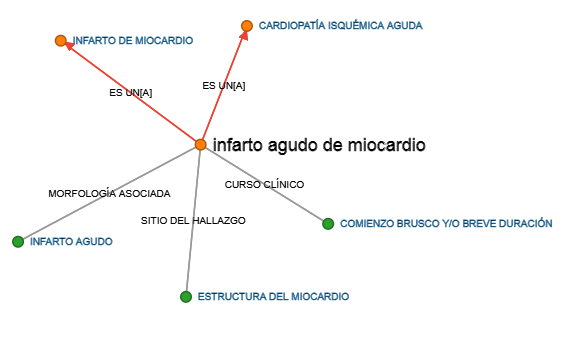
\includegraphics[width=0.9\textwidth]{infarto_agudo_miocardio}
\end{figure}


\subsubsection{Modelo de Conceptos de Snomed CT}
La organización jerárquica de Snomed CT permite pasar de conceptos más genéricos a más específicos \cite{Bhattacharyya2016}. El modelo define la forma en que los conceptos están dispuestos dentro de los subtipos de jerarquía y los tipos de relaciones de atributos que se permiten entre conceptos \cite{Bhattacharyya2016,ihtsdo2016SG}. Como consecuencia, cada concepto debe pertenecer a una sola jerarquía.
% * <mariad.avila@hospitalitaliano.org.ar> 2017-07-02T20:04:44.802Z:
% 
% > grafo dirigido acíclico
% Definir grafo dirigido acíclico en grafos
% 
% ^.
 
Hay 19 jerarquías, no todas son usadas para representar conceptos clínicos. Las siguientes 8 jerarquías tienen reglas para definir atributos y crear conceptos clínicos según \acrshort{IHTSDO} \cite{ihtsdo2016EG}.

\begin{itemize}
\item \textbf{Hallazgo clínico}, representa los resultados de una observación clínica, evaluación o juicio e incluye estados clínicos normales y anormales. La jerarquía de hallazgo clínico incluye conceptos para representar diagnósticos.
\item Los \textbf{procedimientos} representan actividades realizadas en la prestación de servicios de salud. Incluyen no sólo los procedimientos invasivos sino también la administración de medicamentos, toma  de imágenes, educación, terapias y procedimientos administrativos.
\item Los \textbf{especímenes} representan entidades que se obtienen, usualmente de pacientes, para el análisis.
\item \textbf{Estructuras corporales}, representan estructuras anatómicas normales y anormales.
\item \textbf{Productos biológicos/farmacéuticos}, representan productos farmacéuticos (no dispositivos)
\item Las \textbf{situaciones de contexto explícito} representan conceptos en los que el contexto clínico se especifica como parte de una definición del mismo concepto. Esto incluye la presencia o ausencia de una condición, ya sea que el hallazgo clínico es actual, hace parte del pasado o está relacionado a alguien diferente al paciente. Ejemplos de estas situaciones de contexto explicito son: sospecha de cáncer de mama (SCTID: 134405005), antecedente de neoplasia maligna de mama (SCTID: 415076002) y antecedente familiar de neoplasia maligna de mama (SCTID: 429740004), respectivamente.
\item Los \textbf{eventos} representan las ocurrencias que excluyen a los procedimientos y las intervenciones.
\item Por último, los \textbf{objetos físicos }representan a los objetos naturales o hechos por el hombre.
\end{itemize}
 
La tabla \ref{jerarquiasLista} contiene las jerarquías usadas en la lista de problemas y la frecuencia de conceptos de Snomed CT, se puede observar que las jerarquías más usadas son hallazgo clínico, situación con contexto explícito y procedimientos.

% Please add the following required packages to your document preamble:
% \usepackage{booktabs}
\begin{table}[htb]
\centering
\caption{Jerarquías de la lista de problemas y frecuencias de uso}
\label{jerarquiasLista}
\resizebox{\columnwidth}{!}{%
\begin{tabular}{@{}lrr@{}}
\toprule
Jerarquía & Conceptos diferentes & Cantidad de problemas  \\ \midrule
Hallazgo clínico  & \num{82732} & \num{13594650} \\
Situaciones de contexto explícito  & \num{5086} & \num{1222531} \\
Procedimiento & \num{14991} & \num{1138167} \\
Otras Jerarquías  & \num{1122} & \num{144553} \\
Evento & \num{298} & \num{40084}\\
Estructura Corporal  & \num{186} & \num{11274}\\
Producto biológico/farmacéutico & \num{35} & \num{2040} \\
Objeto Físico  & \num{75} & \num{1285} \\ \bottomrule
\end{tabular}
}
\end{table}

\subsubsection{\textit{Reference set}}
\label{par:refset}
Para facilitar el uso de Snomed CT se construyen \textit{\acrfull{refset}}, que son conjuntos de conceptos en determinados dominios como especialidades, cohortes, tipos de enfermedades, etc. Estos dominios se llaman subconjuntos simples.

Uno de los aspectos claves en el uso significativo de la terminología es la creación de \textit{\acrshort{refset}} que puedan ser utilizados como vocabularios controlados para contextos específicos. Estos \textit{\acrshort{refset}} facilitan el uso de Snomed CT como terminología de codificación primaria para la lista de problemas u otros niveles de documentación clínica, y maximizan potencialmente la interoperabilidad de datos a través de las instituciones\cite{Dolin2004KaiserTerminology.}.Snomed CT no define metodologías para construir \textit{\acrshort{refset}} con conceptos que se agrupen por un contexto. La metodología propuesta en esta tesis agrupa los conceptos usados en el registro histórico de la lista de problemas según el contexto dado por el área jerárquica, el grupo etario y el nivel de asistencia con el que fue registrado. 

Existen \textit{\acrshort{refset}} públicos con características similares a los que se analizan en esta tesis. Estos \textit{\acrshort{refset}} fueron compilados por la organización Kaiser Permanente\label{par:kaiser-permanente} con el consenso de todos sus centros médicos\footnote{Kaiser Permanente es la organización de mantenimiento de salud, sin fines de lucro, más grande de los Estados Unidos (integra 28 centros médicos y tiene presencia en 8 estados). Es un sistema integrado de prestación de servicios de salud, que organiza y proporciona o coordina la atención de los miembros de la organización. Kaiser Permanente construyó una solución de terminología médica para toda la organización llamada \textit{\acrfull{CMT}}, que son subconjuntos de terminología adaptada a pacientes y médicos, vinculada a los estándares de interoperabilidad de Estados Unidos e internacionales. Desde el año 2010 donan estos subconjuntos a la \textit{\acrfull{UMLS}}
}. Estos  \textit{\acrshort{refset}} son útiles para hacer comparaciones con los resultantes en los experimentos de este trabajo: \textit{Cardiology; Common Lab Procedures; Emergency Department; Endocrine,  Nephrology, and Urology; ENT, Gastroenterology, and Infectious Diseases; Hematology and Oncology; History and Family History; Injury; Mental Health; Miscellaneous Problem List ; Musculoskeletal; Neurology; Obstetrics and Gynecology; Ophthalmology; Orthopedics; Pediatrics; Primary Care; Radiology; Skin/Dermatology and Respiratory; Specimen Source and Specimen Type; Urology \& Nephrology; Vaccinations; Vascular Procedures List}.


\subsection{Lista de problemas en la \acrshort{HCE} del \acrshort{HIBA} }
\label{par:listaproblemas-HCE}
Cualquier usuario con acceso a la \acrshort{HCE} puede registrar un problema, este usuario puede pertenece a una área administrativa o asistencial del \acrshort{HIBA}. Por consiguiente, las áreas jerárquicas que tiene el \acrshort{HIBA} responden a necesidades operativas de la \acrshort{HCE}, y tienen diferentes niveles de agregación, por ejemplo: Sección de neurocirugía vascular hace parte de una área más general llamada Servicio de neurocirugía. También existen áreas jerárquicas con muy pocos registros o que son \textit{ad hoc} por ejemplo: Instituto universitario H.I., Programa de prevención del cáncer de colon hereditario, Laser en rinosinusología.

Además cada registro de la lista de problemas tiene asociado el nivel de asistencia que indica el ámbito en el que fue cargado el problema. Los niveles de asistencia son las diferentes modalidades de contacto que tiene el paciente con el hospital, asegurando una óptima atención en cada situación específica. En la \acrshort{HCE} el nivel de asistencia puede ser cualquier de los siguientes valores:

\begin{itemize}
\item Ambulatorio: Se tiene definido cuándo empieza y cuándo termina esa atención. El paciente solicita previamente un turno ambulatorio.
\item Episodio ambulatorio: Se sabe cuándo empieza pero no cuándo termina; entonces la modalidad de registro cambia. En el ambulatorio generalmente hay alguien que longitudinalmente ve al paciente en distintos momentos.
\item Triage: Se genera cuando un paciente tiene un contacto con el hospital sin un turno previo, consiste en una revisión médica rápida que permite definir la prioridad de atención.
\item Guardia: Los pacientes críticos con inminencia de muerte o que ingresa con una patología aguda, de gravedad moderada o severa, pero sin muerte inminente por la misma. En este nivel de asistencia se espera que el alta del nivel se dé entre las 24 y 36 horas de su ingreso, pudiendo trasladarse a otro nivel asistencial del hospital, o a otro hospital, o más rara vez a su domicilio.
\item Internación: Tiene un periodo limitado del cuidado, el paciente es tratado por un episodio grave de una enfermedad, cuyas condiciones puedan resultar en un trauma o su muerte. Los tipos de internación son general, domiciliaria y geriátrica.
\end{itemize}


\subsection{Redes}
\subsubsection{Definición}
Las redes están presentes en casi cada aspecto de nuestra vida. La tecnología nos ubica en un mundo lleno de redes, las relaciones físicas o lógicas que establecemos con nuestro entorno constituyen una red en sí misma. Al final de la década del noventa, el avance y popularidad de los computadores cambió la manera como se entendían las redes. La capacidad de los computadores hizo posible acumular grandes bases de datos con estructuras de redes y analizarlas rápida y eficientemente. Esto permitió por primera vez, la comparación de datos de redes reales con los modelos existentes, en particular el modelo ER. Otra influencia importante de la revolución de la computación fue la creación y rápido desarrollo de dos redes enormes: la internet y la World Wide Web (WWW). 

En consecuencia, el concepto abstracto de una red cubre una amplia variedad de estructuras en las cuales las entidades de los sistemas complejos son representados por vértices o nodos y las relaciones o interacciones entre esas entidades son representadas con aristas o enlaces de la red \cite{Estrada2015ATheory}.A continuación presento algunos ejemplos de redes usadas en las áreas de biología y medicina, aunque en la literatura siguen surgiendo nuevos.

\subsubsection{Tipos de redes}
% * <mariad.avila@hospitalitaliano.org.ar> 2017-07-01T16:52:38.003Z:
% 
% Actualizar a 2017
% 
% ^.
 
\paragraph{Redes sociales:} Contempla las redes con interacciones entre individuos. Estos pueden consistir en redes de amigos o conocidos, relaciones de trabajo o sexuales. Además de su importancia en los estudios sociales, entender la estructura de estas redes es también importante para los epidemiólogos, ya que es por medio de estas redes que las epidemias se propagan. \cite{Cohen2010}
 
\paragraph{Redes biológicas:}Este tipo abarca diferentes tipos de redes, las redes biológicas pueden ser lógicas, representando interacciones entre proteínas, entre genes, o entre proteínas y genes. Interacciones entre moléculas en las vías metabólicas de la célula pueden ser vistas como una red. Aunque las interacciones son físicas, los enlaces no son entidades físicas sino la posibilidad de una interacción entre dos moléculas. Otras redes lógicas son las ecológicas predador-presa (donde los vértices son las especies, y los enlaces dirigidos representan la depredación de una especie por la otra). Otro tipo de redes biológicas son las redes biológicas físicas, como el sistema de nervios, las neuronas en el cerebro y la red de venas en un organismo. \cite{Cohen2010}
 
\paragraph{Redes de salud:} A continuación enumero algunos trabajos con redes en el área de la salud.
\begin{itemize}
\item La red de enfermedades humanas \cite{Goh2007TheNetwork.} es una red de trastornos y enfermedades genéticas vinculadas por genes en común. Esta red permite explorar el fenotipo y las enfermedades genéticas asociadas, indicando así el origen genético que tienen en común muchas enfermedades. El proyecto nació en el 2007, y para el 2014 se agregó la red de síntomas a partir de metadata de los encabezados de temas médicos (MeSH\footnote{MeSH por Medical Subject Headings, es el vocabulario controlado Biblioteca Nacional de Medicina. Este vocabulario se usa para indexar artículos para la base de datos MEDLINE y PubMED. Cada cita de los artículos se asocia con un conjunto de palabras claves MeSH que describen el contenido de la cita.}) de PubMED. A partir de estas redes se han hecho múltiples trabajos que explican la interacción entre enfermedades, interacciones entre proteínas, interacciones de enfermedades con drogas y comorbolidades.
\item La red de medicina \cite{Haaren2013,Barabasi2011NetworkDisease}, fue creada  bajo la premisa de que una enfermedad es rara vez consecuencia de una anormalidad en una sola parte del sistema corporal del paciente. Esto implica que las redes deben ilustrar el impacto y la complejidad de la asociación de las enfermedades, además que estás enfermedades pueden ser agrupadas y segmentadas.
\end{itemize}

\subsection{Grafos}
Los grafos se usan para describir de forma matemática relaciones entre redes. Los grafos representan las propiedades topológicas esenciales de una red mediante el tratamiento de ésta como una colección de nodos y enlaces. Este enfoque permite usar herramientas y métodos matemáticos para realizar cálculos en redes complejas.

En su definición es un conjunto de pares ordenados $G=(V,E)$ tal que $E\subseteq [V]^{2}$, así cada elemento de $E$ está asociado a un par de elementos (el mismo o distinto) de $V$. Los elementos de $V$ se llaman vértices (o nodos) de G, y los elementos de $E$ se llaman aristas de G.\cite{Diestel2005GraphTheory,Balakrishnan2000ATheory} 

\subsubsection{Conceptos relacionados a los grafos}

Se comentan y describen algunos términos acerca de grafos, siguiendo las definiciones de Diestel \cite{Diestel2005GraphTheory}:

\paragraph{Orden}
El número de vértices de un grafo, o su cardinalidad, es su \textbf{orden}, y se escribe como $|G|$; el número de aristas se denota con $||G||$. Los grafos son finitos o infinitos de acuerdo a su orden. Un \textbf{grafo vacio} de orden 0 o 1 se llama \textbf{trivial}. Los grafos que se estudian en esta tesis son todos finitos y no triviales.

\paragraph{Adyacencia}
Dos vértices $u$ y $v$ de $G$ son \textbf{adyacentes} o \textbf{vecinos} si $u$ y $v$ son los vértices finales de una arista de $G$. Las dos aristas $e\neq f$ son \textbf{adyacentes} si tienen un vértice en común. 

\paragraph{Grafo completo y triángulo}
Si todos los vértices de $G$ son adyacentes entre si, entonces se dice que $G$ es \textbf{completo}. Un \textbf{grafo completo} de $n$ vértices se denota como $K^{n}$. $K^{3}$ se llama \textbf{triángulo}.

\paragraph{Vértices y aristas independientes}
Los vértices o aristas que no son adyacentes a ningún otro se llaman \textbf{independientes}

\paragraph{Grado}
El \textbf{grado} de un vértice $v$ es el número de $|E(v)|$ de aristas de $v$, es decir el número de vértices adyacentes a $v$. Un vértice de grado 0 es \textbf{independiente}.

\paragraph{Subgrafo}
Sea $G\cup  G':=(V\cup  V', E\cup  E')$ y $G\cap  G':=(V\cap  V', E\cap  E')$. Si $G\cap G' = 0$  entonces $G$ y $G'$ son \textbf{disjuntos}. Si  $V'\subseteq V$ y $E'\subseteq E$, entonces $G'$ es un \textbf{subgrafo} de $G$ (y $G$ es un \textbf{supergrafo} de $G'$), la notación es $G'\subseteq G$. Formalmente se dice que $G$ contiene a $G'$.

\paragraph{Caminos y ciclos}
Un \textbf{camino} es un grafo no trivial $P=(V,E)$ de la forma 
\begin{equation}
V={x_{0},x_{1},...,x_{k}}, E={x_{0}x_{1},x_{1}x_{2},...,x_{k-1}x_{k}}
\end{equation}

donde las $x_{i}$ son todas distintas. Los vértices $x_{0}$ y $x_{k}$ están enlazados por $P$ y se llaman vértices \textbf{terminales}. Los vértices $x_{1},...,x_{k-1}$ son los vértices \textbf{internos} de $P$. El número de aristas de un camino es su \textbf{longitud}.

Si $P=x_{0}...x_{k-1}$ es un camino y $k\geq 3$, entonces el grafo $C:=P+x_{k-1}x_{0}$ se llama un \textbf{ciclo}. Se denomina ciclo por su (cíclica) secuencia de vértices, el ciclo anterior se escribe como $x_{0}...x_{k-1}x_{0}$.

\paragraph{Grafos dirigidos}
Un \textbf{grafo dirigido} es un par $(V,E)$ de conjuntos disjuntos de vértices y aristas que juntos formas dos mapas (1) inicial: $E\rightarrow V$ y (2) terminal: $E\rightarrow V$, asignándole a cada arista $e$ un \textbf{vértice inicial} $inicial(e)$ y un \textbf{vértice termina}l $terminal(e)$. Se dice que la arista $e$ se dirige desde $inicial(e)$ a $terminal(e)$.

\paragraph{Grafo de Snomed CT}
Al diseccionar la estructura de Snomed CT, cada concepto se representa con un vértice y cada relación entre los conceptos se representa por una arista. No hay relaciones circulares y todas son unidireccionales sin excepciones, pero un vértice $inicial(e)$ puede tener más de una relación de salida o vértices $terminal(e)$, de esta manera se construye un grafo acíclico dirigido. \cite{Bhattacharyya2016}

\subsubsection{Patrones de grafos en redes}
La mayoría de las redes de gran escala comparten patrones que no se notan en redes pequeñas. Entre todos los patrones, la mayoría de las características más conocidas son: \textbf{distribución libre de escala, efecto de mundo pequeño y fuertes estructuras de comunidad}.\cite{Tang2010}

\paragraph{Distribución libre de escala} \cite{Tang2010}.
\label{par:definicion-libre-escala}
Los grados de los vértices en las redes de gran escala a menudo siguen una distribución de ley de potencia, también conocidas como distribución Zipfian o distribución Pareto. 

En su definición, una variable aleatoria $X$ sigue una distribución de ley de potencia si
\begin{equation}
p(x)=Cx^{-\alpha}, x\geq  x_{min}; \alpha \geq 1
\end{equation}

De tal manera que $\alpha \geq 1$ asegura que exista una constante de normalización $C$. Una distribución que sigue la ley de potencia se llama también  distribución sin escalas, ya que la forma de la distribución permanece sin cambios, excepto para una constante multiplicativa general, cuando la escala de unidades se incrementa por un factor. Esto es
\begin{equation}
p(ax)=bp(x)
\end{equation}
 
Donde $a$ y $b$ son constantes. En otras palabras, no existe una escala característica con la variable aleatoria. La forma funcional es la misma para todas las escalas. La red con una distribución libre de escalas para los grados nodales también se denomina \textbf{red libre de escala}.
 
Mientras que para las distribuciones normales, es extremadamente raro que un evento ocurra con una desviación muy lejana de la media, en las distribuciones de ley de potencias la cola es mucho más larga. De tal manera es común que algunos vértices de la red tengan alto grado mientras que la mayoría tengan pocas conexiones. La razón es que la cola de una distribución de ley de potencias decae polinomialmente. Esto es asintotáticamente más lento que en la distribución normal que lo hace exponencialmente, resultando en un fenómeno de cola pesada. La curva de la distribución de ley de potencias se convierte en una recta si graficamos la distribución en una escala log-log, ya que
\begin{equation}
\log p(x) =-\alpha \log x + \log C
\end{equation}
Esta asociación se puede usar para verificar graficamente si la distribución sigue la ley de potencias. Una verificación más robusta es aproximar la función de \acrfull{cdf} descripta con la siguiente ecuación:
\begin{equation}
F(X\geq x) \propto  x^{-\alpha+1 }
\end{equation}

\paragraph{Métricas de comunidades}
\label{par:efecto-comunidades}
Informalmente, una comunidad es un conjunto de vértices donde cada vértice es más cercano a otros vértices en su comunidad que a los vértices que están fuera de ella. Esta característica ha sido encontrado especialmente en las redes sociales \cite{Tang2010}. La figura \ref{fig:ejemploCluster} ilustra las comunidades que se forman a partir de las relaciones de los vértices, cada color representa una comunidad.

\begin{figure}
\caption{Ejemplo de comunidades}
\label{fig:ejemploCluster}
\centering
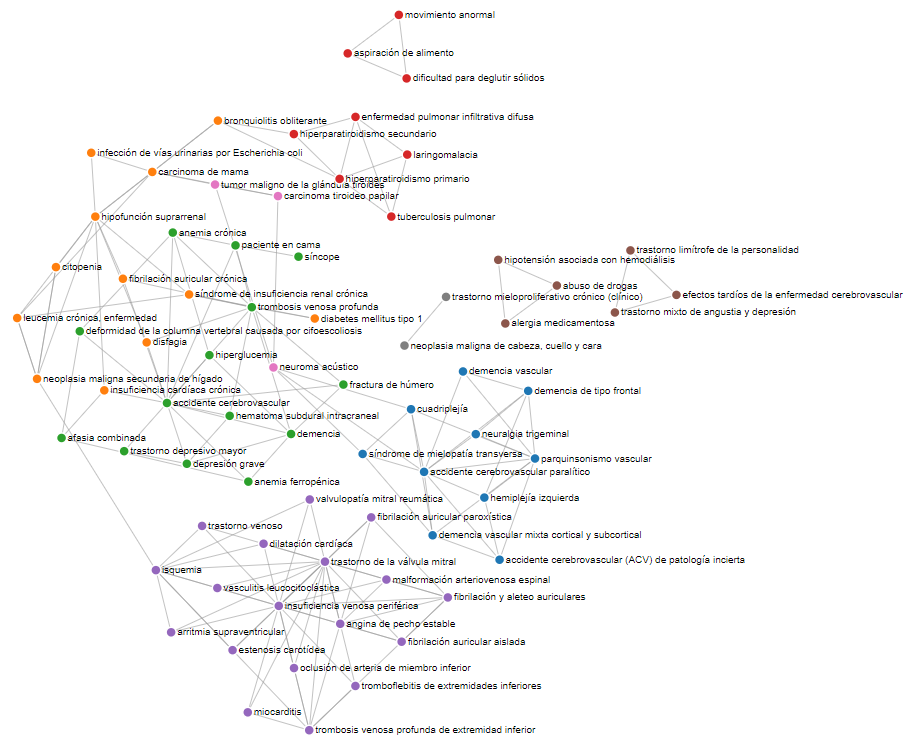
\includegraphics[width=\textwidth]{ejemplo_cluster.png}
\end{figure}

La fuerza de las comunidades se miden con diferentes métricas, en esta tesis se analiza el coeficiente de agrupamiento global o \textbf{transitividad}, el coeficiente de agrupamiento promedio y la longitud media del camino mínimo entre vértices. 

\subparagraph{Coeficiente de agrupamiento - Transitividad}
La transitividad \cite{Wasserman1994} $C^{\Delta}$, se calcula como una medida de la proporción de triángulos cerrados en un grafo:
\begin{equation}
\label{equ:coeficiente_transitividad}
C^{\Delta} =3x\frac{\text{número de triángulos}}{\text{número de tripletas conectadas}}
\end{equation}
Esta métrica muestra de manera global cuán agrupado es el grafo, ya que representa la probabilidad de que dos vértices estén conectados si comparten un vecino en común. En el contexto de la lista de problemas, si los problemas $P1$, $P2$ co-ocurren en pacientes que también tengan $P3$, esta métrica representa la probabilidad de que $P1$ y $P2$ ocurran juntas.

\subparagraph{Coeficiente de agrupamiento - Promedio}\cite{Saramaki2006,Kaiser2008}
El promedio del coeficiente de agrupamiento del grafo G, necesita del cálculo local de los coeficientes de agrupamiento de cada vértice i,

\begin{equation}
c_{i} = \frac{\Gamma_{v_{i}}}{|E(v_{i})|(|E(v_{i})|-1)},
\end{equation}

donde $|E(v_{i})|$ es el grado del vértice $v_{i}$ y $\Gamma_{v_{i}}$ es el número de aristas entre los vecinos de $v_{i}$.

Finalmente, el coeficiente de agrupamiento se calcula con la siguiente ecuación.
\begin{equation}
\label{equ:coeficiente_promedio}
C = \frac{1}{n}\sum_{v \in G} c_v,
\end{equation}

El coeficiente de agrupamiento promedio produce una alta varianza para los vértices con menos grados. Por ejemplo, para vértices con grado 2, $C_{i}$ es 0 o 1.\cite{Tang2010} %%Se usa comúnmente para estudios numéricos mientras que la \textbf{transitividad} se utiliza más para el estudio analítico.%%

La figura \ref{fig:ejemplocoeficienteagrupamiento} muestra en los ejemplos a), b) y c) el cálculo del coeficiente de agrupamiento del vértice i en azul. En el ejemplo d) está el cálculo de cada nodo. Siguiendo las ecuaciones \ref{equ:coeficiente_promedio} y \ref{equ:coeficiente_transitividad}, el coeficiente de agrupamiento promedio es de \num{0.310} y la transitividad es de \num{0.375}, respectivamente.

\begin{figure}
\caption{Ejemplos de coeficientes de agrupamiento}
\label{fig:ejemplocoeficienteagrupamiento}
\centering
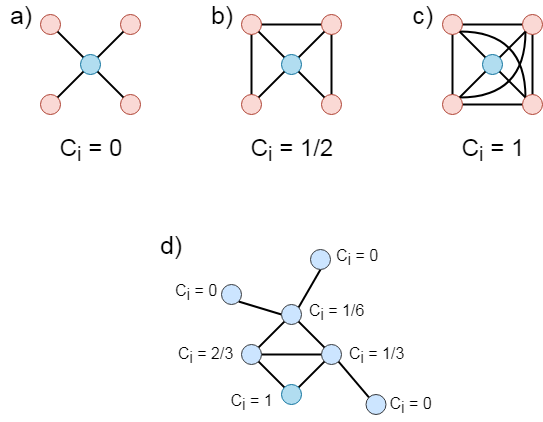
\includegraphics[width=0.8\textwidth]{Images/coeficiente_de_agrupamiento.png}
\end{figure}

\subparagraph{Longitud media del camino mínimo entre vértices}
Cálculo de la media de la distancia entre los vértices en un grafo. Comunidades con longitudes medias más pequeñas indican estructuras de comunidades más fuertes.

\subparagraph{Distancia semántica}
La distancia semántica se usa para calcular similaridad entre conceptos. En diferentes trabajos en el dominio médico \cite{Wang2010,Gan2013,Pedersen2007,Zare2015ASNOMED-CT} se presentan diferentes maneras más sofisticadas de calcular la similaridad que la longitud media del camino mínimo. Sin embargo, estos enfoques son también alguna variante de la longitud media del camino mínimo.
El modelo de datos define la arista "$|\text{ES UN}|$" para establecer relaciones entre conceptos ancestros y descendientes, de tal manera que todos los conceptos son un subtipo de otro más general, y un concepto puede tener uno o más descendientes con varios niveles de especificación.

\begin{figure}[ht]
\caption{Modelo de datos}
\label{fig:distancias_semanticas}
\centering
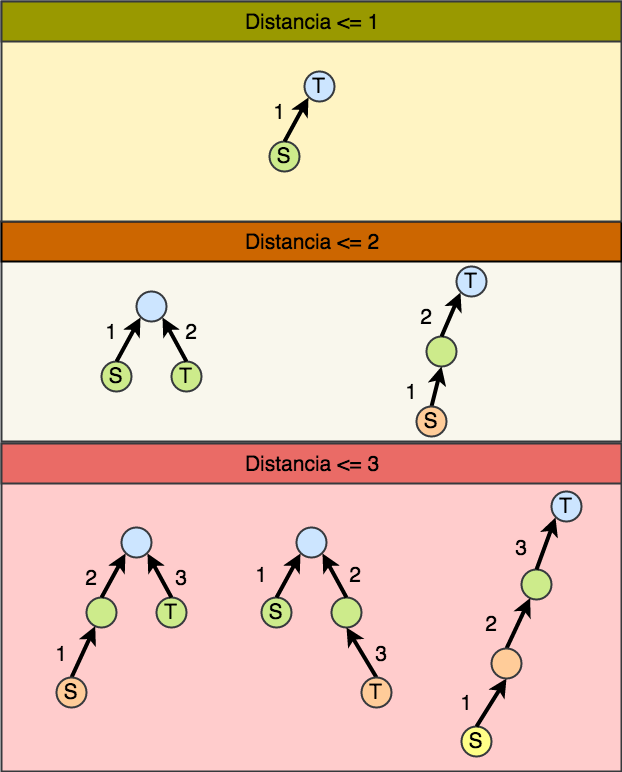
\includegraphics[width=0.5\textwidth]{distancias_semanticas}
\end{figure}


\subsection{\textit{Graphmining}}
La minería de datos se ha convertido en sinónimo de encontrar patrones frecuentes en datos transaccionales, el término más general descubrimiento de conocimiento abarca esta y otras tareas. Descubrimiento o aprendizaje no supervisado en \textit{graphmining} implica no sólo la tarea de encontrar patrones en un conjunto de transacciones, sino también encontrar la posible superposición de patrones en un gran grafo. Descubrimiento también implica la tarea de \textbf{\textit{clustering}}, la cual intenta describir todos los datos por medio de la identificación clases de grafos que comparten patrones comunes de atributos y relaciones entre si. \textit{Clustering} también puede extraer relaciones entre \textit{clusters}, resultando en una organización jerárquica o taxonómica.\cite{Cook2006}
 
En contraste, el aprendizaje supervisado es la tarea de extraer patrones que distinguen un conjunto de otros. Estos conjuntos se llaman los ejemplos positivos y los negativos. Este conjunto de ejemplos pueden contener muchas transacciones de grafos o un sólo gran grafo. El objetivo es encontrar un patrón de relación entre nodos que aparezca a menudo en los ejemplos positivos pero no en los ejemplos negativos. Tal patrón se usa para predecir la clase (positiva o negativa) de nuevos ejemplos. \cite{Cook2006}
 
La última tarea en graph mining es la visualización del conocimiento descubierto. La visualización de grafos es la representación de los vértices, aristas y etiquetas de un grafo de tal manera que los humanos entiendan los conceptos representados por el grafo.\cite{Cook2006}

\subsubsection{Análisis de redes}
El análisis de redes involucra una variedad de tareas \cite{Tang2010}, a continuación listo las que aplicaré en este trabajo:

\begin{enumerate}
  \item Análisis de centralidad, ayuda a identificar los vértices (o problemas en el contexto de esta tesis) “más importantes” en la red. Esta importancia puede definirse de distinta manera y cada una ayuda a entender diferentes aspecto de la influencia y el poder del vértice en la red:
  
\begin{itemize}
\item \textbf{Centralidad de grado.}
Cuenta el número de conexiones que tiene un vértice. Los problemas con los grados más altos serán los que más ocurren en los pacientes.
\item \textbf{Intermediación (\textit{betweenness}).} Mide el número de veces que un vértice en particular es miembro de los caminos más cortos entre otros dos vértices.
Usualmente, la medida de intermediación está normalizada en el rango de [0, 1], dónde 0 es un vértice desconectado y 1 un vértice por donde pasan todas las conexiones.\cite{Cook2006,Brath2015GraphData}
\item \textbf{Cercanía (\textit{Closeness}).} La cercanía de un vértice mide la distancia promedio a todos los otros vértices. Si pocos vértices son alcanzables o si la distancia entre los vértices aumenta, entonces la medida de cercanía es pequeña. \cite{Cook2006,Brath2015GraphData}.
\item \textbf{Centralidad de autovector (\textit{Eigenvector}).} Dado un vértice, se suma recursivamente todas las distancias a todos los otros vértices. Entre más centrales sean los otros vértices, el vértice que se está midiendo tendrá mayor centralidad\cite{Brath2015GraphData}.
\end{itemize}
\item Clasificación de redes y detección de \textit{outliers}. Algunos problemas están etiquetados con información contextual: servicio de salud, ámbito y grupo etario. Por ejemplo, en una red con algunos problemas pocos comunes identificados como del Servicio Cardiológico, ¿es posible inferir otros problemas poco comunes asociados por su co-ocurrencia en los pacientes?
  \item \textit{Clustering}. Según Blonde et al.\cite{Blondel2008FastNetworks}, el problema de \textit{clustering} requiere la partición de una red en grupos de vértices densamente conectados, donde los vértices que pertenecen a diferentes grupos se conectan escasamente. Las formulaciones exactas de este problema de optimización son computacionalmente intratables. En los últimos años se han propuesto muchos algoritmos para encontrar particiones razonablemente buenas de una manera razonablemente rápida, debido al incremento de la disponibilidad de conjuntos de datos con grandes redes y el impacto de las redes en la vida. Se pueden distinguir los siguientes tipos de algoritmos \label{par:algoritmos-nosupervisados}:
.
\begin{itemize}
\item \textbf{Divisivos:} Se comienza con todo el grafo y se van eliminando iterativamente las aristas, dividiendo así progresivamente el grafo en subgrafos desconectados más y más pequeños. Estos subgrafos se identifican como comunidades. El punto crucial en un algoritmo divisivo es la selección de las aristas que se van a eliminar, las cuales deben ser las que conectan comunidades y no las aristas que están dentro de las comunidades. \cite{Radicchi2004DefiningNetworks,Girvan2002CommunityNetworks.,Newman2004FastNetworks}
\item \textbf{Aglomerativos:} Para cada uno de los vértices del grafo se calcula un peso, el cual mide qué tan conectados están los vértices. A partir del conjunto de todos los vértices sin aristas, se ordenan decrecientemente los vértices según su pesos, y se agregan iterativamente las aristas entre pares similares de vértices. De esta manera, los vértices se agrupan en comunidades cada vez más grandes, y el árbol se construye hasta la raíz. Este árbol representa a todo el grafo. \cite{Radicchi2004DefiningNetworks,Pons2005ComputingWalks}
\item \textbf{Optimización:} Estos algoritmos buscan encontrar resultados usando heurísticas o maximizando una función objetivo con un enfoque voraz (\textit{greedy}) para mejorar la complejidad computacional de los algoritmos clásicos. Estos métodos consisten en unir recursivamente las comunidades buscando optimizar la función objetivo.\cite{Clauset2004FindingNetworks,Blondel2008FastNetworks}
\end{itemize}
  
\end{enumerate}

\subsubsection{Evaluación de estructuras}
La detección de comunidades es el tópico que se desarrolla en mayor profundidad en esta tesis. Se usan los tres enfoques principales y se comparan los resultados. En parte, la razón por la cual hay tantas definiciones y métodos, es que no está clara cómo debe ser la estructura de una comunidad en una red real. De tal manera que diferentes métodos se desarrollaron según las necesidades de sus autores \cite{Tang2010}.

Para poder comparar los diferentes resultados obtenidos con los algoritmos, utilizaré las siguientes estrategias:

\begin{itemize}
\item Cálculo de modularidad
\item Comparación de las comunidades con un \textit{gold-standard }
\end{itemize}

\paragraph{Cálculo de modularidad.}
 
Según Newman \cite{Newman2006FindingMatrices.}, una buena división de una red en comunidades no es solamente aquella en la que el número de aristas  entre los grupos es pequeño, sino en la que el número de aristas entre los grupos es menor al esperado. Sólo si el número de aristas entre los grupos es significativamente más bajo al esperado se puede decir con justificación que se ha encontrado una estructura de comunidad significativa. Equivalentemente, se puede examinar el número de aristas dentro de las comunidades y buscar divisiones de las redes en las cuales este número es más alto del esperado, los dos enfoques son equivalentes. Estas consideraciones constituyen una medida basada en un punto de corte para modificar una función de beneficio $Q$ definida como
\begin{equation}
Q =  (\text{Número de aristas en la comunidad}) -  (\text{Número de aristas esperadas})
\end{equation} 

Esta función de beneficio se llama \textbf{modularidad}. La modularidad de una partición es un valor escalar entre -1 y 1. La modularidad mide la densidad de los enlaces en las comunidades comparándola con los enlaces entre las comunidades\cite{Blondel2008FastNetworks}. Valores cercanos a 1 indican estructuras de comunidades más fuertes, y valores cercanos a -1 indican que los nodos están agrupados en comunidades a las que no pertenecen\cite{Tang2010}.

\paragraph{Comparación de las comunidades con un \textit{gold-standard}.}
\label{par:cubrimiento}

El término \textit{gold-standard} \cite{Versi1992quotGoldTerm.} se utiliza en los trabajos científicos para referirse a valores de referencia que están disponible en condiciones razonables. No es la prueba perfecta, sino la mejor disponible. El \textit{gold-standard} es importante ante la imposibilidad de realizar mediciones directas para determinar si los conceptos que están dentro de una comunidad realmente pertenecen o no a ella. Los \textit{gold-standard} con el que se realizan las mediciones son los públicos y disponibles por la organización Kaiser Permanente (Ver sección \ref{par:kaiser-permanente}).

La medición que se realizo se llama cubrimiento, la cual se define como la proporción de los conceptos que se comparten entre los dos conjuntos de datos, al tamaño del \textit{\acrshort{refset}} (Ver sección \ref{par:refset}) de referencia $T$, como se define en la ecuación \ref{eq:cubrimiento}

\begin{equation}\label{eq:cubrimiento}
\textup{cubrimiento} = \frac{\textup{conceptos mapeados en T}}{\textup{Tamaño de T}}
\end{equation}

\begin{itemize}
\item \textit{Conceptos mapeados en T}, es el número total de conceptos de Snomed CT que comparten el \textit{refset} que se compara y el \textit{refset} $T$, y
\item el \textit{tamaño de T} es el número total de conceptos que tiene el \textit{refset} $T$.
\end{itemize}

\section{Objetivos}
Con el presente trabajo se contribuye a la organización de los datos y el uso significativo de Snomed CT para la recuperación de información en la lista de problemas del Hospital Italiano de Buenos Aires. Esta contribución es la construcción de una taxonomía de problemas, cuyas relaciones son ponderadas por su co-ocurrencia en las listas de problemas de los pacientes y sus relaciones jerárquicas con Snomed CT.

El producto final de este trabajo es el modelo que representa grupos o clasificaciones y las relaciones significativas de los problemas que co-ocurren en los pacientes. Los experimentos para llegar a este modelo tendrán en cuenta la lista de problemas y se añadirá  información de contexto: ámbito o nivel de asistencia, área jerárquica y grupo etario. La comparación entre los modelos y la evaluación de su capacidad predictiva se hará con las medidas de precisión y exactitud. 

\section{Organización del trabajo}
% * <mariad.avila@hospitalitaliano.org.ar> 2017-07-01T16:27:48.600Z:
% 
% Cómo va a estar organizada la tesis
% 
% ^.
En el capítulo 2 se explica la metodología, se describen los algoritmos y los criterios de evaluación.

En el capítulo 3 hago una descripción de los datos y las decisiones en la limpieza de datos. Luego, se aplican las técnicas de \textit{graphmining}.
 
Por último en el capítulo 4, hablo sobre las conclusiones y futuros pasos.
